%! TEX root = ../main.tex

\section{Arquitectura general}
\label{sec:solucion}

\observacion{Esta sección 7 deberá empezar con una descripción general (gráfico)
y debe ir explicando parte por parte}

A continuación se describe la arquitectura propuesta para la realización de una
juego serio, \fixme{se utiliza}{} la guía básica definida
por~\cite{pereira2009design} y descrita en~\ref{sec:desarrollo}.

Esta sección se enfoca en los aspectos técnicos de la creación del juego serio,
las competencias básicas relacionadas con la educación (segundo paso de la guía
descrita en~\ref{sec:desarrollo}) se definieron en las
secciones~\ref{sec:glasgow} y~\ref{sec:hemocultivo}.

La solución se basa en escena\fixme{s, u}{}na escena es un procedimiento definido
en~\ref{sec:seleccion_escenas}, cada escena tiene sus propias entidades, eventos
y requisitos específicos. \fixme{Adicionalmente existe otra escena denominada
Inicio que es la escena donde se inicia la solución.}{?}
%Inicio estaba en un \enquote

\observacion{Grafo de la arquitectura? Esta un poco desordenado}

Adicionalmente la solución cuenta con pantallas, que son vistas donde el usuario
puede seleccionar varias opciones, a continuación se describe el funcionamiento
global de la solución y la transición entre las escenas, pantallas y diversas
opciones existentes. Posteriormente se define como se interactúa con el entorno,
y a continuación se evalúa al alumno durante su experiencia con la solución.

\subsection{Flujo de la solución}

\observacion{Mejorar siguiente parrafo}
La solución consiste varios escenarios, y cada escenario, \fixme{existen}{Se
    presenta?} varias pantallas que muestran información relevante de acuerdo a
la situación de la simulación, la figura~\ref{fig:grafo_estados} es una
representación abstracta de este flujo de acciones disponibles dentro de la
solución.

\begin{figure}[H] 
\centering 
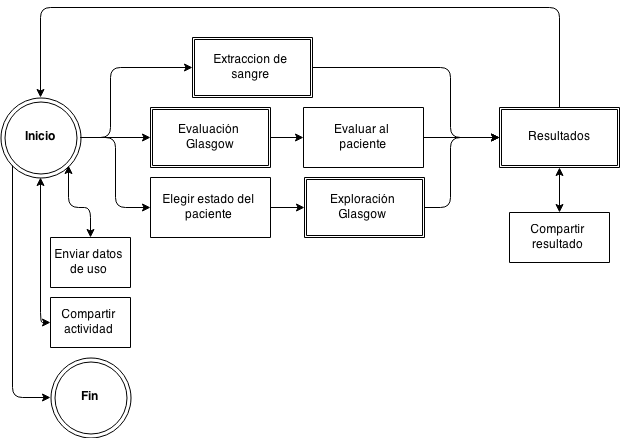
\includegraphics[scale=0.5]{solucion/images/grafo_escenas.png}
\caption{Diagrama de navegación entre los distintos escenarios y pantallas
    disponibles en la solución.}
\label{fig:grafo_estados}
\end{figure}

 
La figura~\ref{fig:grafo_estados} muestra que la solución empieza con una escena
denominada \emph{Inicio}. En la pantalla \emph{Inicio} se observa el escenario y 
opciones, que conducen a los escenarios \emph{Extracción de Sangre} y
\emph{Glasgow}. Otras opciones incluidos en el escenario \emph{Inicio} son
\begin{enumerate*}[label=\itshape\alph*\upshape)]
\item enviar datos de uso al \emph{backend},
\item iniciar sesión en el \emph{Facebook}, y,
\item salir de la simulación.
\end{enumerate*}


\fixme{El escenario \emph{Extracción de Sangre} finaliza al presionar la opción
\emph{Finalizar Partida} y luego se muestra la pantalla \emph{Resultados}, con
información de retroalimentación y la opciones de compartir resultado y volver
a la escena \emph{Inicio}.}{Finalizar }

Para iniciar el escenario \emph{Glasgow} existen dos caminos:
\begin{enumerate}
\item \textbf{Explorar}: desde la escena \emph{Inicio} se elige la opción \emph{Explorar
        Glasgow} en ese momento se muestra la pantalla \emph{Elegir estado del
        paciente}, donde se personaliza el estado del paciente y luego se inicia
    la escena. La escena finaliza con la opción \emph{Finalizar Partida} y se
    muestra la pantalla \emph{Resultados}.
\item \textbf{Evaluar}: desde la escena \emph{Inicio} se elige la opción \emph{Evaluar
        Glasgow} y se inicia la escena \emph{Glasgow} con un estado del paciente
    aleatorio.
    Al finalizar la escena, se muestra la pantalla \emph{Evaluar al paciente}
    donde se permite elegir el estado del paciente, y luego se pasa a la
    pantalla \emph{Resultados}
\end{enumerate}

Finalmente, en la pantalla \emph{Resultados} se permite compartir resultado y
volver a la escena \emph{Inicio}.

Todos los escenarios son utilizados de manera similar, la interacción con la
escena es siempre la misma.

\subsection{Transformaciones del punto de vista del usuario}

El usuario se desenvuelve en un entorno de tres dimensiones, en el cual realiza
las actividades relacionadas a la práctica, se distinguen dos tipos de acciones
principales que el usuario puede realizar:

\begin{itemize}
    \item \textbf{Alejamiento o acercamiento}: es el acto de acercar o alejar la
        cámara, y por consiguiente al usuario del paciente. Se realiza
        utilizando dos dedos, para realizar un acercamiento, mientras se
        mantiene presionada la pantalla con ambos dedos, se procede a alejar un
        dedo del otro, para realizar un alejamiento, se debe acercar ambos
        dedos.
    \item \textbf{Rotación}: se refiere al movimiento de rotación alrededor de
        un foco, que en ambas escenas es el paciente, para realizarla, se utiliza
        un dedo, y se mueve el dedo en cualquier dirección, la cámara, se moverá
        en la dirección contraria.
\end{itemize}

\subsection{Evaluación del usuario}
\label{sec:eca_impl}

\todo[backgroundcolor=white,inline,caption={Pregunta}]{Si esto esta flotando acá
    es por que no sabemos donde podemos poner los detalles de implementación del
    Motor, no se ponen en la parte de extracción de sangre para mantener la
    consistencia con glasgow.}

En la sección~\ref{sec:eca} se describen los \Gls{eca}, y los mismos son
utilizados para poder realizar la evaluación del alumno en la solución.

Definir si las acciones de un usuario son correctas utilizando un motor
\Gls{eca} es sencillo teniendo en cuenta que sólo se deben definir un
conjunto de acciones que se deben realizar, y agregar una acción que verifica si
los pasos realizados fueron los correctos.

Se describe como se crean las reglas, de manera a explicar como son utilizadas
para la evaluación de las acciones realizadas por el usuario.

La definición de las reglas se realiza de la siguiente forma:

\begin{algorithm}[H]
\caption{Creación de regla de verificación de calzado de guantes}
\label{alg:rule_guante}
\lstset{style=sharpc}
\begin{lstlisting}
Rule.New().
     When(``enfermero.guantes.calzar'').
     Then(enviroment => enviroment.
            estadoPaciente.TieneManosLimpias()).
\end{lstlisting}
\end{algorithm}

La regla del algoritmo~\ref{alg:rule_guante} controla que el estudiante ha
realizado la acción \enquote{Calzarse los guantes}, y en ese momento tenga las
manos limpias.

\subsubsection{Estados de una regla}
\observacion{Hacer referencia a la figura 7.2 o mover adelante (la figura del
    ciclo de vida)}

Una regla puede estar en uno de los siguientes estados:

\begin{enumerate}
\item \textbf{BEGIN} Es una regla que recién fue creada, no realiza ninguna
	acción.
\item \textbf{WAITING\_FOR\_RULE:} Es un estado en el que esta esperando que otras reglas
	sean lanzadas. En este estado, es un suscriptor de las reglas por la que
	espera, y no forma parte del ciclo de ejecución del motor de reglas.
\item \textbf{WAITING\_FOR\_EVENT:} Es un estado en el que esta escuchando que sean
	lanzados los eventos a los que escucha, este es el estado principal. En
	este estado, es un suscriptor de los eventos por los que espera, y no
	forma parte del ciclo de ejecución del motor de reglas.
\item \textbf{WAITING\_FOR\_CONDITION:} La regla ya no espera por ningún evento y las
	reglas de las que depende ya han sido lanzadas, se verifica cada cierto
	tiempo si el entorno cumple con una condición definida. 
\item \textbf{FINISH:} Estado final de una regla.
\end{enumerate}

\begin{figure}
\centering
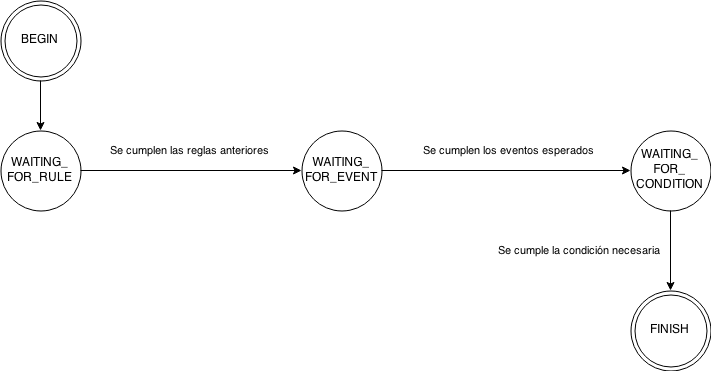
\includegraphics[width=12cm]{solucion/images/rules_flow.png}
\caption{Ciclo de vida de una regla}
\label{fig:rule_flow}
\end{figure}

En la figura~\ref{fig:rule_flow} se observa la evolución de una regla, es
importante notar que una regla solo puede avanzar en este flujo.

\subsubsection{Motor de ejecución}

Un motor de reglas \gls{eca}, requiere de un proceso que evalúe constantemente
las reglas para verificar si las mismas deben ser lanzadas o
no\cite{bailey2004event,galton2002two}, un algoritmo comúnmente utilizado para
realizar la verificación es el algoritmo de \enquote{RETE}\revisar{Tener el
    algoritmo en la presentación, como anexo}\cite{de2001eca}, la cantidad de
reglas definidas, y la no dependencia circular entre ellas, hace innecesario la
implementación de tal algoritmo\cite{de2001eca}. 

De acuerdo a la descripción dada en~\ref{sec:eca_ejecucion}, la propuesta
implementada utiliza una ejecución inmediata, principalmente por la sencillez
de las reglas, es decir, las reglas no realizan un proceso complejo, solamente
controlan el estado del entorno y lo validan.

Además, la ejecución inmediata es importante por que el entorno no sufre
modificaciones entre el evento lanzado y la ejecución de la regla, según
\cite{bailey2004event}, este es el factor más importante para determinar el tipo
de ejecución deseado.

El motor de reglas actúa sobre aquellas reglas en estado
\emph{WAITING\_FOR\_CONDITION} e invoca al procedimiento que se encarga de
validar si la regla puede ser activada (el procedimiento es único por cada
regla), si el mismo determina que la regla puede ser lanzada, el motor ejecuta
la acción de la regla y modifica el estado de la regla a \emph{FINISH}.

%A continuación, se describen todos los escenarios, primeramente se da una
%descripción general de los escenarios y se procede a explicar los detalles de
%los mismos, incluyendo las entidades, eventos y acciones que pueden ser
%realizados en el mismo.
